%% SECTION HEADER /////////////////////////////////////////////////////////////////////////////////////
\section{Predictions of FCN pixel-wise segmentation models}
\label{sec52}

%% SECTION CONTENT ////////////////////////////////////////////////////////////////////////////////////

%% SUBSECTION HEADER //////////////////////////////////////////////////////////////////////////////////
\subsection{Numerical cases}
\label{sec521}
In this section, five FCN models, including Res-UNet, VGG16 encoder-decoder, FCN-DenseNet, PSPNet, and GCN, were evaluated on four selected damage cases of an RMS (from the bottom surface of the plate).

The first exemplary delamination case is shown in Fig.~\ref{fig:rms_first_case}. 
The delamination is located at the left edge of the plate, and it is surrounded by a line to represent its shape and location as shown in Fig.~\ref{fig:RMS_bottom_448}.
Figures~\ref{fig:unet_269}-~\ref{fig:gcn_269} show the predicted output of the Res-UNet, VGG16 encoder-decoder, PSPNet, FCN-DenseNet and GCN models, respectively. 
%%%%%%%%%%%%%%%%%%%%%%%%%%%%%%%%%%%%%%%%%%%%%%%%%%%%%%%%%%%%%%%%%%%%%%%%%%%%%%%%
All models properly indicate the location of the delamination. 
Moreover, pixels related to delamination location are clustered into a single spot without any additional noise. 
The GCN model better visually resembles the actual shape of the delamination than other models.
%%%%%%%%%%%%%%%%%%%%%%%%%%%%%%%%%%%%%%%%%%%%%%%%%%%%%%%%%%%%%%%%%%%%%%%%%%%%%%%%
% First case
%%%%%%%%%%%%%%%%%%%%%%%%%%%%%%%%%%%%%%%%%%%%%%%%%%%%%%%%%%%%%%%%%%%%%%%%%%%%%%%%
\begin{figure} [!h]
	\centering
	\begin{subfigure}[b]{.48\textwidth}
		\centering
		\includegraphics[width=.9\textwidth]{Figures/Chapter_5/RMS_flat_shell_Vz_448_500x500bottom.png}
		\caption{RMS \& Label.}
		\label{fig:RMS_bottom_448}
	\end{subfigure}
	\hfill
	\begin{subfigure}[b]{.48\textwidth}
		\centering
		\includegraphics[width=.9\textwidth]{Figures/Chapter_5/UNet_num_269.png}
		\caption{Res-UNet.}
		\label{fig:unet_269}	
	\end{subfigure}
	\hfill
	\begin{subfigure}[b]{.48\textwidth}
		\centering
		\includegraphics[width=0.9\textwidth]{Figures/Chapter_5/VGG16_autoencoder_269.png}
		\caption{VGG16 encoder-decoder.}
		\label{fig:vgg16_269}
	\end{subfigure}
	\hfill
	\begin{subfigure}[b]{.48\textwidth}
		\centering
		\includegraphics[width=0.9\textwidth]{Figures/Chapter_5/PSPNet_269.png}
		\caption{PSPNet.}
		\label{fig:pspnet_269}	
	\end{subfigure}
	\hfill
	\begin{subfigure}[b]{.48\textwidth}
		\centering
		\includegraphics[width=0.9\textwidth]{Figures/Chapter_5/FCN_DenseNet_269.png}
		\caption{FCN-DenseNet.}
		\label{fig:densenet_269}
	\end{subfigure}
	\hfill
	\begin{subfigure}[b]{.48\textwidth}
		\centering
		\includegraphics[width=0.9\textwidth]{Figures/Chapter_5/GCN_269.png}
		\caption{GCN.}
		\label{fig:gcn_269}	
	\end{subfigure}
	\caption{First delamination case based on numerical data.}
	\label{fig:rms_first_case}
\end{figure}

%%%%%%%%%%%%%%%%%%%%%%%%%%%%%%%%%%%%%%%%%%%%%%%%%%%%%%%%%%%%%%%%%%%%%%%%%%%%%%%%
In the second delamination case, shown in Fig.~\ref{fig:rms_second_case}, the delamination is located at the upper left corner of the plate, and it is surrounded by an ellipse to represent its shape and location as shown in Fig.~\ref{fig:RMS_bottom_456}.
%%%%%%%%%%%%%%%%%%%%%%%%%%%%%%%%%%%%%%%%%%%%%%%%%%%%%%%%%%%%%%%%%%%%%%%%%%%%%%%%
This is the most challenging damage scenario because of reflections coming from plate edges overshadows reflections from damage.
As a result, changes in RMS patterns are barely visible.
%%%%%%%%%%%%%%%%%%%%%%%%%%%%%%%%%%%%%%%%%%%%%%%%%%%%%%%%%%%%%%%%%%%%%%%%%%%%%%%%
Figures~\ref{fig:unet_301} -~\ref{fig:gcn_301} show the predicted output of the Res-UNet, VGG16 encoder-decoder, PSPNet, FCN-DenseNet and GCN models, respectively. 
%%%%%%%%%%%%%%%%%%%%%%%%%%%%%%%%%%%%%%%%%%%%%%%%%%%%%%%%%%%%%%%%%%%%%%%%%%%%%%%%
In this delamination case the PSPNet model were not able to identify the damage.
However, the rest models perform reasonably well, considering the difficult damage scenario.
%%%%%%%%%%%%%%%%%%%%%%%%%%%%%%%%%%%%%%%%%%%%%%%%%%%%%%%%%%%%%%%%%%%%%%%%%%%%%%%%
% Second case
%%%%%%%%%%%%%%%%%%%%%%%%%%%%%%%%%%%%%%%%%%%%%%%%%%%%%%%%%%%%%%%%%%%%%%%%%%%%%%%%
\begin{figure} [!h]
	\centering
	\begin{subfigure}[b]{.48\textwidth}
		\centering
		\includegraphics[width=0.9\textwidth]{Figures/Chapter_5/RMS_flat_shell_Vz_456_500x500bottom.png}
		\caption{RMS \& Label.}
		\label{fig:RMS_bottom_456}
	\end{subfigure}
	\hfill
	\begin{subfigure}[b]{.48\textwidth}
		\centering
		\includegraphics[width=0.9\textwidth]{Figures/Chapter_5/UNet_num_301.png}
		\caption{Res-UNet.}
		\label{fig:unet_301}	
	\end{subfigure}
	\hfill
	\begin{subfigure}[b]{.48\textwidth}
		\centering
		\includegraphics[width=0.9\textwidth]{Figures/Chapter_5/VGG16_autoencoder_301.png}
		\caption{VGG16 encoder-decoder.}
		\label{fig:vgg16_301}
	\end{subfigure}
	\hfill
	\begin{subfigure}[b]{.48\textwidth}
		\centering
		\includegraphics[width=0.9\textwidth]{Figures/Chapter_5/PSPNet_301.png}
		\caption{PSPNet.}
		\label{fig:pspnet_301}	
	\end{subfigure}
	\hfill
	\begin{subfigure}[b]{.48\textwidth}
		\centering
		\includegraphics[width=0.9\textwidth]{Figures/Chapter_5/FCN_DenseNet_301.png}
		\caption{FCN-DenseNet.}
		\label{fig:densenet_301}
	\end{subfigure}
	\hfill
	\begin{subfigure}[b]{.48\textwidth}
		\centering
		\includegraphics[width=0.9\textwidth]{Figures/Chapter_5/GCN_301.png}
		\caption{GCN.}
		\label{fig:gcn_301}	
	\end{subfigure}
	\caption{Second delamination case based on numerical data.}
	\label{fig:rms_second_case}
\end{figure}

%%%%%%%%%%%%%%%%%%%%%%%%%%%%%%%%%%%%%%%%%%%%%%%%%%%%%%%%%%%%%%%%%%%%%%%%%%%%%%%%

The third delamination case is shown in Figure~\ref{fig:rms_third_case}. 
The delamination is located at the upper middle of the plate and it is surrounded by an ellipse to represent its shape and location as shown in Fig.~\ref{fig:RMS_bottom_438}.
Figures~\ref{fig:unet_229} -~\ref{fig:gcn_229} show the predicted output of the Res-UNet, VGG16 encoder-decoder, PSPNet, FCN-DenseNet and GCN models, respectively. 
%%%%%%%%%%%%%%%%%%%%%%%%%%%%%%%%%%%%%%%%%%%%%%%%%%%%%%%%%%%%%%%%%%%%%%%%%%%%%%%%
In this case, the elliptical shape of delamination is best preserved by Res-UNet and FCN-DenseNet. 
%However, the highest value of IoU is obtained by GCN (see Table~\ref{tab:table_numerical_scenarios})
%%%%%%%%%%%%%%%%%%%%%%%%%%%%%%%%%%%%%%%%%%%%%%%%%%%%%%%%%%%%%%%%%%%%%%%%%%%%%%%%
% Third case
%%%%%%%%%%%%%%%%%%%%%%%%%%%%%%%%%%%%%%%%%%%%%%%%%%%%%%%%%%%%%%%%%%%%%%%%%%%%%%%%
\begin{figure} [!h]
	\centering
	\begin{subfigure}[b]{.48\textwidth}
		\centering
		\includegraphics[width=0.9\textwidth]{Figures/Chapter_5/RMS_flat_shell_Vz_438_500x500bottom.png}
		\caption{RMS \& Label.}
		\label{fig:RMS_bottom_438}
	\end{subfigure}
	\hfill
	\begin{subfigure}[b]{.48\textwidth}
		\centering
		\includegraphics[width=0.9\textwidth]{Figures/Chapter_5/UNet_num_229.png}
		\caption{Res-UNet.}
		\label{fig:unet_229}	
	\end{subfigure}
	\hfill
	\begin{subfigure}[b]{.48\textwidth}
		\centering
		\includegraphics[width=0.9\textwidth]{Figures/Chapter_5/VGG16_autoencoder_229.png}
		\caption{VGG16 encoder-decoder.}
		\label{fig:vgg16_229}
	\end{subfigure}
	\hfill
	\begin{subfigure}[b]{.48\textwidth}
		\centering
		\includegraphics[width=0.9\textwidth]{Figures/Chapter_5/PSPNet_229.png}
		\caption{PSPNet.}
		\label{fig:pspnet_229}	
	\end{subfigure}
	\hfill
	\begin{subfigure}[b]{.48\textwidth}
		\centering
		\includegraphics[width=0.9\textwidth]{Figures/Chapter_5/FCN_DenseNet_229.png}
		\caption{FCN-DenseNet.}
		\label{fig:densenet_229}
	\end{subfigure}
	\hfill
	\begin{subfigure}[b]{.48\textwidth}
		\centering
		\includegraphics[width=0.9\textwidth]{Figures/Chapter_5/GCN_229.png}
		\caption{GCN.}
		\label{fig:gcn_229}	
	\end{subfigure}
	\caption{Third delamination case based on numerical data.}
	\label{fig:rms_third_case}
\end{figure}

%%%%%%%%%%%%%%%%%%%%%%%%%%%%%%%%%%%%%%%%%%%%%%%%%%%%%%%%%%%%%%%%%%%%%%%%%%%%%%%%
In the fourth delamination case, shown in Fig.~\ref{fig:rms_fourth_case}, the delamination is located at the upper left quarter of the plate, and it is surrounded by an ellipse to represent its shape and location as shown in Fig.~\ref{fig:RMS_bottom_397}.
%%%%%%%%%%%%%%%%%%%%%%%%%%%%%%%%%%%%%%%%%%%%%%%%%%%%%%%%%%%%%%%%%%%%%%%%%%%%%%%%
Figures~\ref{fig:unet_65} -~\ref{fig:gcn_65} show the predicted output of the Res-UNet, VGG16 encoder-decoder, PSPNet, FCN-DenseNet and GCN models, respectively. 
%%%%%%%%%%%%%%%%%%%%%%%%%%%%%%%%%%%%%%%%%%%%%%%%%%%%%%%%%%%%%%%%%%%%%%%%%%%%%%%%
All models perform reasonably well for this damage case.
%%%%%%%%%%%%%%%%%%%%%%%%%%%%%%%%%%%%%%%%%%%%%%%%%%%%%%%%%%%%%%%%%%%%%%%%%%%%%%%%
% Fourth case
%%%%%%%%%%%%%%%%%%%%%%%%%%%%%%%%%%%%%%%%%%%%%%%%%%%%%%%%%%%%%%%%%%%%%%%%%%%%%%%%
\begin{figure} [!h]
	\centering
	\begin{subfigure}[b]{.48\textwidth}
		\centering
		\includegraphics[width=0.9\textwidth]{Figures/Chapter_5/RMS_flat_shell_Vz_397_500x500bottom.png}
		\caption{RMS \& Label.}
		\label{fig:RMS_bottom_397}
	\end{subfigure}
	\hfill
	\begin{subfigure}[b]{.48\textwidth}
		\centering
		\includegraphics[width=0.9\textwidth]{Figures/Chapter_5/UNet_num_65.png}
		\caption{Res-UNet.}
		\label{fig:unet_65}	
	\end{subfigure}
	\hfill
	\begin{subfigure}[b]{.48\textwidth}
		\centering
		\includegraphics[width=0.9\textwidth]{Figures/Chapter_5/VGG16_autoencoder_65.png}
		\caption{VGG16 encoder-decoder.}
		\label{fig:vgg16_65}
	\end{subfigure}
	\hfill
	\begin{subfigure}[b]{.48\textwidth}
		\centering
		\includegraphics[width=0.9\textwidth]{Figures/Chapter_5/PSPNet_65.png}
		\caption{PSPNet.}
		\label{fig:pspnet_65}	
	\end{subfigure}
	\hfill
	\begin{subfigure}[b]{.48\textwidth}
		\centering
		\includegraphics[width=0.9\textwidth]{Figures/Chapter_5/FCN_DenseNet_65.png}
		\caption{FCN-DenseNet.}
		\label{fig:densenet_65}
	\end{subfigure}
	\hfill
	\begin{subfigure}[b]{.48\textwidth}
		\centering
		\includegraphics[width=0.9\textwidth]{Figures/Chapter_5/GCN_65.png}
		\caption{GCN.}
		\label{fig:gcn_65}	
	\end{subfigure}
	\caption{Fourth delamination case based on numerical data.}
	\label{fig:rms_fourth_case}
\end{figure}
\clearpage

%%%%%%%%%%%%%%%%%%%%%%%%%%%%%%%%%%%%%%%%%%%%%%%%%%%%%%%%%%%%%%%%%%%%%%%%%%%%%%%%
Table~\ref{tab:RMS_num_cases} presents the evaluation metrics for all FCN models, regarding the numerical cases shown in Figs.~\ref{fig:rms_first_case},~\ref{fig:rms_second_case},~\ref{fig:rms_third_case}, and~\ref{fig:rms_fourth_case}.
Table~\ref{tab:RMS_num_cases} gathers the actual delamination area \(A\), predicted delamination area \(\hat{A}\), intersection over union IoU and percentage area error \(\epsilon\) with respect to each case. 
The overall performance of the GCN model is better than other models for the selected delamination scenarios.
%%%%%%%%%%%%%%%%%%%%%%%%%%%%%%%%%%%%%%%%%%%%%%%%%%%%%%%%%%%%%%%%%%%%%%%%%%%%%%%%
\begin{table}[ht!]
	\centering
	\caption{Evaluation metrics of the four numerical cases.}
	\label{tab:RMS_num_cases}
	\begin{tabular}{cccccc}
		\toprule[1.5pt]
		\multirow{2}{*}{Model} & \multirow{2}{*}{case number} & \multicolumn{1}{c}{\multirow{2}{*}{A [mm\textsuperscript{2}]}} & \multicolumn{3}{c}{Predicted output} \\ 
		\cmidrule(lr){4-6} & & & \multicolumn{1}{c}{IoU} & \multicolumn{1}{c}{\(\hat{A}\) [mm\textsuperscript{2}]} & \(\epsilon\) \\
		\midrule
		\multirow{4}{*}{Res-UNet} 
		& 1 & 717 & \multicolumn{1}{c}{0.50} & \multicolumn{1}{c}{402} & \(43.93\%\) \\ 
		& 2 & 257 & \multicolumn{1}{c}{0.45} & \multicolumn{1}{c}{143} & \(44.36\%\) \\ 
		& 3 & 105 & \multicolumn{1}{c}{0.67} & \multicolumn{1}{c}{88} & \(16.19\%\) \\ 
		& 4 & 537 & \multicolumn{1}{c}{0.80} & \multicolumn{1}{c}{478} & \(10.99\%\) \\ 
		\midrule
		\multirow{4}{*}{VGG16 encoder-decoder} 
		& 1 & 717 & \multicolumn{1}{c}{0.51} & \multicolumn{1}{c}{410} & \(42.82\%\) \\ 
		& 2 & 257 & \multicolumn{1}{c}{0.69} & \multicolumn{1}{c}{203} & \(21.01\%\) \\ 
		& 3 & 105 & \multicolumn{1}{c}{0.75} & \multicolumn{1}{c}{117} & \(11.43\%\) \\ 
		& 4 & 537 & \multicolumn{1}{c}{0.65} & \multicolumn{1}{c}{385} & \(28.31\%\) \\ 
		\midrule
		\multirow{4}{*}{FCN-DenseNet} 
		& 1 & 717 & \multicolumn{1}{c}{0.73} & \multicolumn{1}{c}{1073} & \(49.65\%\) \\ 
		& 2 & 257 & \multicolumn{1}{c}{0.52} & \multicolumn{1}{c}{505} & \(96.50\%\) \\ 
		& 3 & 105 & \multicolumn{1}{c}{0.66} & \multicolumn{1}{c}{118} & \(12.38\%\) \\ 
		& 4 & 537 & \multicolumn{1}{c}{0.72} & \multicolumn{1}{c}{815} & \(51.77\%\) \\ 
		\midrule
		\multirow{4}{*}{PSPNet} 
		& 1 & 717 & \multicolumn{1}{c}{0.39} & \multicolumn{1}{c}{596} & \(16.88\%\) \\ 
		& 2 & 257 & \multicolumn{1}{c}{0.00} & \multicolumn{1}{c}{0} & \(-\%\) \\ 
		& 3 & 105 & \multicolumn{1}{c}{0.44} & \multicolumn{1}{c}{156} & \(48.57\%\) \\ 
		& 4 & 537 & \multicolumn{1}{c}{0.77} & \multicolumn{1}{c}{610} & \(13.59\%\) \\ 
		\midrule
		\multirow{4}{*}{GCN} 
		& 1 & 717 & \multicolumn{1}{c}{0.79} & \multicolumn{1}{c}{666} & \(7.11\%\) \\ 
		& 2 & 257 & \multicolumn{1}{c}{0.71} & \multicolumn{1}{c}{215} & \(16.34\%\) \\ 
		& 3 & 105 & \multicolumn{1}{c}{0.72} & \multicolumn{1}{c}{177} & \(68.57\%\) \\ 
		& 4 & 537 & \multicolumn{1}{c}{0.86} & \multicolumn{1}{c}{523} & \(2.61\%\) \\ 
		\bottomrule[1.5pt]
	\end{tabular}	
\end{table}
%%%%%%%%%%%%%%%%%%%%%%%%%%%%%%%%%%%%%%%%%%%%%%%%%%%%%%%%%%%%%%%%%%%%%%%%%%%%%%%%

Table~\ref{tab:table_all_numerical_cases} presents the mean and maximum values of IoU calculated for the previously unseen numerical test set for all FCN models.
Table~\ref{tab:table_all_numerical_cases} shows that all models have a relatively high IoU, indicating their ability to detect and localise the delamination.
%, which is higher compared to the traditional signal processing techniques such as the adaptive wavenumber filtering presented in our previous work~\cite{Ijjeh2021}. 
%The mean \(IoU\) for the adaptive wavenumber filtering technique regarding the whole testing samples was \(0.373\) compared to the previous FCN-DenseNet model, which has a mean \(IoU\) of \(0.623\).
%%%%%%%%%%%%%%%%%%%%%%%%%%%%%%%%%%%%%%%%%%%%%%%%%%%%%%%%%%%%%%%%%%%%%%%%%%%%%%%%
\begin{table}[ht!]
	\centering
	\caption{Analysis of numerical cases.}
	\label{tab:table_all_numerical_cases}	
	\begin{tabular}{lcc}
		\toprule
		Model & mean \(IoU\) & max \(IoU\) \\ 
		\midrule 
		Res-UNet & \(0.66\) & \(0.89\) \\ 
		VGG16 encoder-decoder & \(0.57\) & \(0.84\) \\ 
		FCN-DenseNet & \(0.68\) & \(0.92\) \\ 
		PSPNet & \(0.55\) & \(0.91\) \\ 
		GCN & \(0.76\) & \(0.93\) \\ 
		\bottomrule
	\end{tabular}
	
\end{table}
%%%%%%%%%%%%%%%%%%%%%%%%%%%%%%%%%%%%%%%%%%%%%%%%%%%%%%%%%%%%%%%%%%%%%%%%%%%%%%%%
%%%%%%%%%%%%%%%%%%%%%%%%%%%%%%%%%%%%%%%%%%%%%%%%%%%%%%%%%%%%%%%%%%%%%%%%%%%%%%%%%
%\begin{table}[ht!]
%	\centering
%	\caption{Model parameters}
%	\label{tab:table_parameters}
%	{
%		\begin{tabular}{lc}
%			\toprule
%			Model & Total parameters ($\approx$) \\ 
%			\midrule 
%			Res-UNet & \(52\times 10^{6}\) \\ 
%			VGG16 encoder-decoder & \(37.3\times 10^{6}\) \\ 
%			FCN-DenseNet & \(2.5\times 10^{6}\) \\ 
%			PSPNet & \(6.6\times 10^{6}\) \\ 
%			GCN & \(36\times 10^{6}\) \\ 
%			\bottomrule
%		\end{tabular}
%	}
%\end{table}
\clearpage
%%%%%%%%%%%%%%%%%%%%%%%%%%%%%%%%%%%%%%%%%%%%%%%%%%%%%%%%%%%%%%%%%%%%%%%%%%%%%%%%
\subsection{Experimental cases}
\label{sec522}

In this section, FCN models are evaluated using experimentally acquired data.
%%%%%%%%%%%%%%%%%%%%%%%%%%%%%%%%%%%%%%%%%%%%%%%%%%%%%%%%%%%%%%%%%%%%%%%%%%%%%%%%
Similarly to the synthetic dataset, we applied a frequency of \(50\)~kHz to excite a signal in a transducer placed at the centre of the plate. 
\(A0\) mode wavelength for this particular CFRP material at such frequency is about \(19.5\)~mm. 
The measurements were performed by using Polytec PSV-\(400\) SLDV on the bottom surface of the plate with dimensions of \(500\times 500\)~mm. 
The measurements were conducted on a regular grid of \(333\times333\) points. 
The measurement area was aligned with the plate edges.
The sampling frequency was \(512\)~kHz.
The experimental case is for a CFRP specimen with a single delamination.
A plain weave fabric reinforcement was used for manufacturing the composite specimen. 
The delamination between layers of the fabric was created artificially by a Teflon insert of a thickness 250 $\mu$m. 
The Teflon of a square shape was inserted during specimen manufacturing, so its shape and location are known. 
The number of full wavefield frames for this case is $f_n = 256$.
Furthermore, the measured full wavefield was further processed by an energy compensated RMS which takes into account wave attenuation. 
The results of such operation are shown in Fig.~\ref{fig:ERMS_with_label}.
The delamination is surrounded by a square frame representing its shape and location. 
Figures~(\ref{fig:unet_exp_erms} - \ref{fig:gcn_exp_erms}) shows delamination prediction maps for Res-UNet, VGG16 encoder-decoder, PSPNet, FCN-DenseNet and GCN models, receptively.
%%%%%%%%%%%%%%%%%%%%%%%%%%%%%%%%%%%%%%%%%%%%%%%%%%%%%%%%%%%%%%%%%%%%%%%%%%%%%%%%

Table~\ref{tab:rms_exp_case} presents the evaluation metrics for all FCN models, regarding the experimental case shown in Figs.~\ref{fig:exp_erms__case}.
Table~\ref{tab:rms_exp_case} gathers the actual delamination area \(A\), predicted delamination area \(\hat{A}\), intersection over union IoU and percentage area error \(\epsilon\) with respect to each FCN model. 
The overall performance of the GCN model is better than other models for the selected delamination scenarios.
Similarly to the numerical dataset, the best accuracy was achieved by using GCN.
%%%%%%%%%%%%%%%%%%%%%%%%%%%%%%%%%%%%%%%%%%%%%%%%%%%%%%%%%%%%%%%%%%%%%%%%%%%%%%%%
%%%%%%%%%%%%%%%%%%%%%%%%%%%%%%%%%%%%%%%%%%%%%%%%%%%%%%%%%%%%%%%%%%%%%%%%%%%%%%%
\begin{table}[!ht]
	\centering
	\caption{Evaluation metrics of the experimental case.}
	\label{tab:rms_exp_case}
	\begin{tabular}{lcccc}
		\toprule
		\multirow{2}{*}{Model} & \multicolumn{1}{c}{\multirow{2}{*}{A [mm\textsuperscript{2}]}} & \multicolumn{3}{c}{Predicted output} \\ 
		\cmidrule(lr){3-5} & & \multicolumn{1}{c}{IoU} & \multicolumn{1}{c}{\(\hat{A}\) [mm\textsuperscript{2}]} & \(\epsilon\) \\ \midrule
		Res-UNet & \multirow{5}{*}{210} & \multicolumn{1}{c}{0.58} & \multicolumn{1}{c}{323}  & \(53.8\%\) \\ 
		VGG16 encoder-decoder &  & \multicolumn{1}{c}{0.62} & \multicolumn{1}{c}{320} & \(52.4\%\) 
		\\ 
		FCN-DenseNet &  & \multicolumn{1}{c}{0.54} & \multicolumn{1}{c}{386} & \(83.8\%\) \\ 
		PSPNet &  & \multicolumn{1}{c}{0.49} & \multicolumn{1}{c}{580} & \(176.2\%\) 
		\\ 
		GCN &  & \multicolumn{1}{c}{0.72} & \multicolumn{1}{c}{309} & \(47.1\%\) 
		\\ 
		\bottomrule
	\end{tabular}		
\end{table}
%%%%%%%%%%%%%%%%%%%%%%%%%%%%%%%%%%%%%%%%%%%%%%%%%%%%%%%%%%%%%%%%%%%%%%%%%%%%%%%%
\begin{figure} [!h]
	\centering
	\begin{subfigure}[b]{.48\textwidth}
		\centering
		\includegraphics[width=0.9\textwidth]{Figures/Chapter_5/ERMS_with_label.png}
		\caption{ERMS CFRP Teflon inserted \& Label.}
		\label{fig:ERMS_with_label}
	\end{subfigure}
	\hfill
	\begin{subfigure}[b]{.48\textwidth}
		\centering
		\includegraphics[width=0.9\textwidth]{Figures/Chapter_5/Fig_UNET_7.png}
		\caption{Res-UNet.}
		\label{fig:unet_exp_erms}	
	\end{subfigure}
	\hfill
	\begin{subfigure}[b]{.48\textwidth}
		\centering
		\includegraphics[width=0.9\textwidth]{Figures/Chapter_5/Fig_VGG16_7.png}
		\caption{VGG16 encoder-decoder.}
		\label{fig:vgg16_exp_erms}
	\end{subfigure}
	\hfill
	\begin{subfigure}[b]{.48\textwidth}
		\centering
		\includegraphics[width=0.9\textwidth]{Figures/Chapter_5/Fig_PSPNET_7.png}
		\caption{PSPNet.}
		\label{fig:pspnet_exp_erms}	
	\end{subfigure}
	\hfill
	\begin{subfigure}[b]{.48\textwidth}
		\centering
		\includegraphics[width=0.9\textwidth]{Figures/Chapter_5/Fig_FCN_DenseNet_7.png}
		\caption{FCN-DenseNet.}
		\label{fig:densenet_exp_erms}
	\end{subfigure}
	\hfill
	\begin{subfigure}[b]{.48\textwidth}
		\centering
		\includegraphics[width=0.9\textwidth]{Figures/Chapter_5/Fig_GCN_7.png}
		\caption{GCN.}
		\label{fig:gcn_exp_erms}	
	\end{subfigure}
	\caption{Fourth delamination case based on numerical data.}
	\label{fig:exp_erms__case}
\end{figure}


It should be noted that the developed FCN-DenseNet model presented in~\cite{Ijjeh2021} was compared to the conventional adaptive wavenumber filtering method presented in~\cite{Kudela2015, Radzienski2019}.

%Furthermore, the FCN-DenseNet model showed better performance in delamination identification for numerical cases.
The FCN models show good generalisation behaviour in predicting the delamination in the unseen numerically generated data.
We can observe that the models can identify delamination with nearly no noise, indicating that the models can generalize and detect delamination on previously unseen data.
It has been shown that the achieved accuracy of the FCN models presented in~\cite{Ijjeh2022} surpasses the accuracy of previous models in~\cite{Ijjeh2021} with an improvement of 22.47\%.
Given that the provided models were only trained on a numerically generated dataset, they had a high degree of generalisation.
Additionally, the models show their ability to generalise by detecting the delamination in the experimentally acquired data.

Figure~\ref{fig:exp_erms_case_comp} presents a comparison between the predicted outputs regarding the experi\-mental case with the adaptive wavenumber filtering presented in~\cite{Kudela2015, Radzienski2019} and the two versions of the developed FCN-DenseNet models presented in~\cite{Ijjeh2021} and~\cite{Ijjeh2022}, respectively.
Figure.~\ref{fig:ERMSF} shows the damage map represents the energy-based root mean square index of frames filtered in the wavenumber domain (ERMSF).
To eliminate low values from the ERMSF, a binary threshold is applied as shown in Fig.~\ref{fig:Binary_ERMSF}.
The threshold level was set to minimise the influence of edge noise while still highlighting the damage.
The calculated IoU equals $0.401$.
Figure.~\ref{fig:FCN_densenet_2021} shows the predicted output for the developed FCN-DenseNet model in~\cite{Ijjeh2021}, and the calculated IoU equals $0.081$. 
Fig.~\ref{fig:FCN_densenet_2022} shows the predicted output of the improved FCN-DenseNet model developed in~\cite{Ijjeh2022}, and the calculated IoU equals to $0.54$.
Accordingly, the improved version of the FCN-DenseNet model developed in~\cite{Ijjeh2022} surpasses both the adaptive wavenumber filtering method and the FCN-DenseNet model developed in~\cite{Ijjeh2021}.
%%%%%%%%%%%%%%%%%%%%%%%%%%%%%%%%%%%%%%%%%%%%%%%%%%%%%%%%%%%%%%%%%%%%%%%%%%%%%%%%
\begin{figure} [!h]
	\centering
	\begin{subfigure}[b]{.48\textwidth}
		\centering
		\includegraphics[width=0.7\textwidth]{Figures/Chapter_5/ERMSF_CFRP_teflon_3o_375_375p_50kHz_5HC_x12_15Vpp.png}
		\caption{ERMSF.}
		\label{fig:ERMSF}
	\end{subfigure}
	\hfill
	\begin{subfigure}[b]{.48\textwidth}
		\centering
		\includegraphics[width=0.7\textwidth]{Figures/Chapter_5/Binary_ERMSF_CFRP_teflon_3o_375_375p_50kHz_5HC_x12_15Vpp.png}
		\caption{Binary ERMSF.}
		\label{fig:Binary_ERMSF}	
	\end{subfigure}
	\hfill
	\begin{subfigure}[b]{.48\textwidth}
		\centering
		\includegraphics[width=0.7\textwidth]{Figures/Chapter_5/Predicted_Predicted_ERMS_CFRP_teflon_3o_375_375p_50kHz_5HC_x12_15Vpp_7_softmax.png}
		\caption{FCN-DenseNet~\cite{Ijjeh2021}}
		\label{fig:FCN_densenet_2021}
	\end{subfigure}
	\hfill
	\begin{subfigure}[b]{.48\textwidth}
		\centering
		\includegraphics[width=0.7\textwidth]{Figures/Chapter_5/Fig_FCN_DenseNet_7.png}
		\caption{FCN-DenseNet~\cite{Ijjeh2022}}
		\label{fig:FCN_densenet_2022}	
	\end{subfigure}
	\caption{Comparsion of the experimental case by using the adaptive wavenumber filtering method~\cite{Kudela2015, Radzienski2019}, FCN-DenseNet~\cite{Ijjeh2021}, FCN-DenseNet~\cite{Ijjeh2022}.}
	\label{fig:exp_erms_case_comp}
\end{figure}

